
\afterpage{%
	\clearpage
	\newgeometry{margin=0.5cm}
	\begin{landscape}
		\thispagestyle{empty}
		\begin{figure}[h]
			\begin{subfigure}{.49\linewidth}
				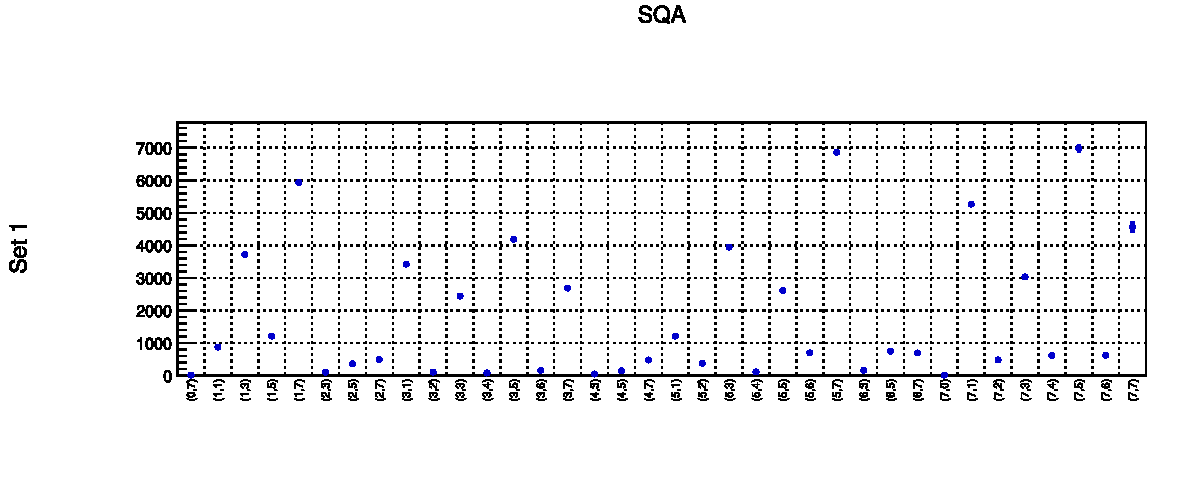
\includegraphics[width=1.08\linewidth]{Pictures/1}
			\end{subfigure}
			\hspace{-.73cm}
			\begin{subfigure}{.49\linewidth}
				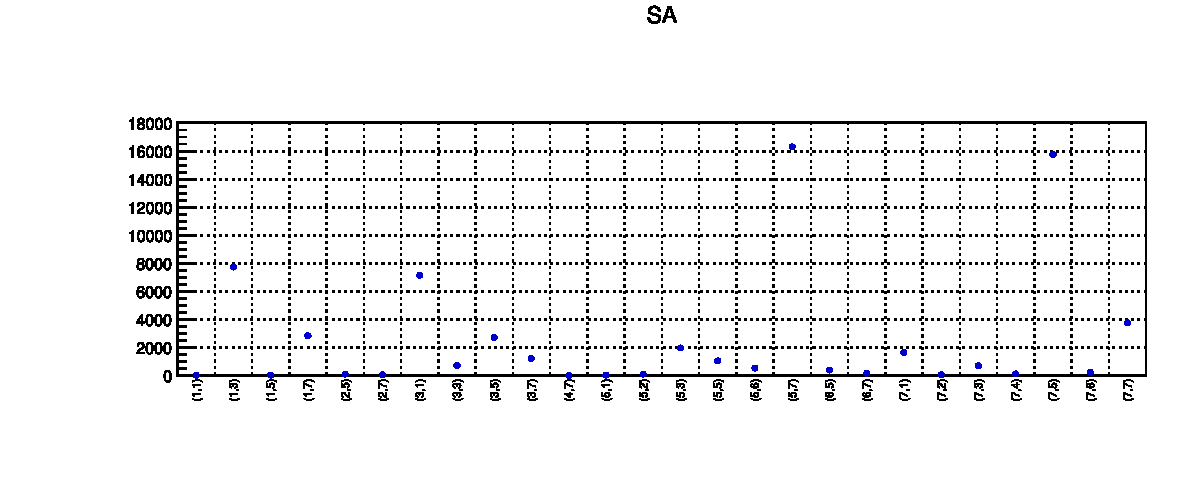
\includegraphics[width=1.08\linewidth]{Pictures/2}
			\end{subfigure}
			
			\vspace{-1.8cm}
			\begin{subfigure}{.49\linewidth}
				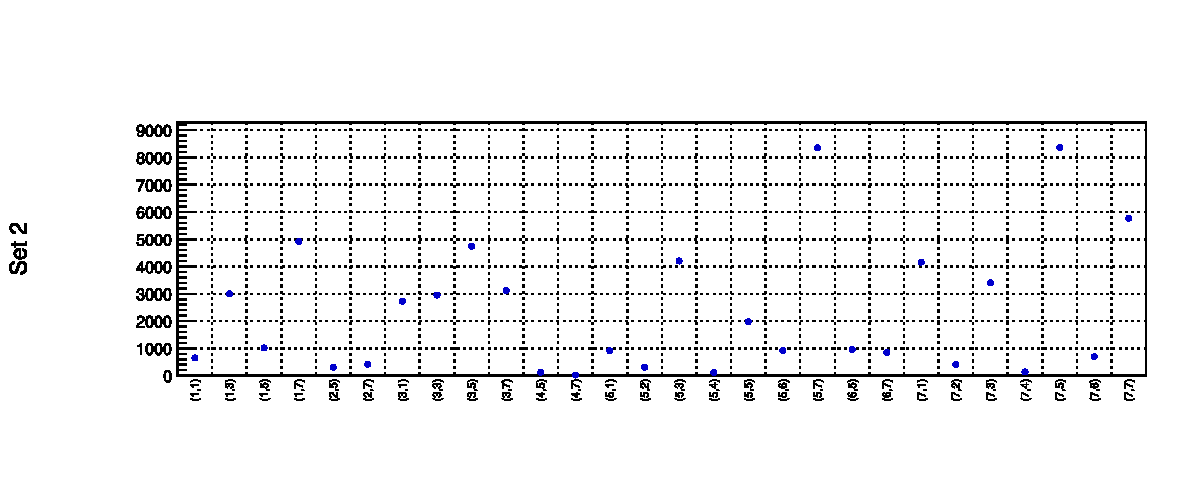
\includegraphics[width=1.08\linewidth]{Pictures/3}
			\end{subfigure}
			\hspace{-.73cm}
			\begin{subfigure}{.49\linewidth}
				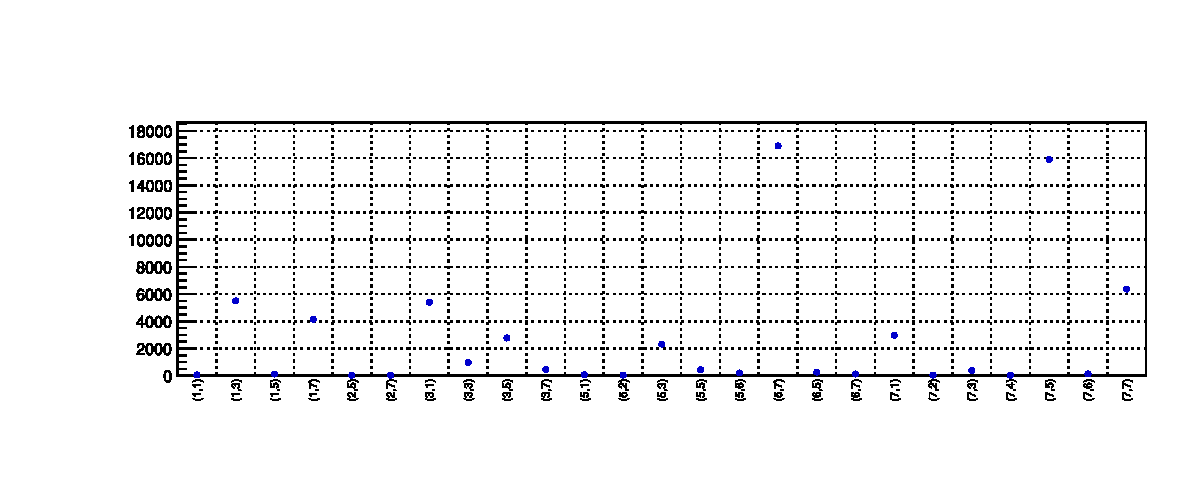
\includegraphics[width=1.08\linewidth]{Pictures/4}
			\end{subfigure}
			
			\vspace{-1.8cm}
			\begin{subfigure}{.49\linewidth}
				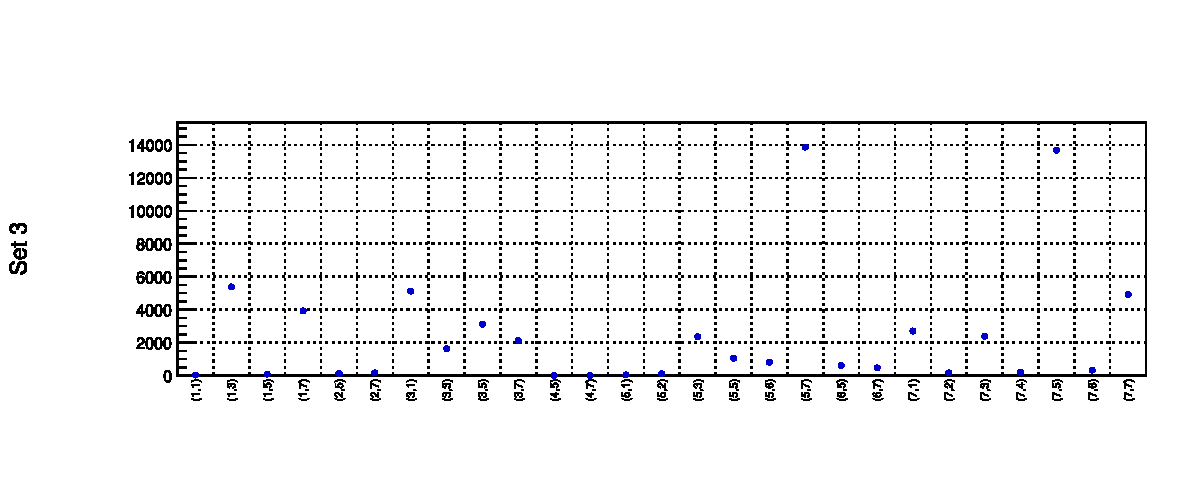
\includegraphics[width=1.08\linewidth]{Pictures/5}
			\end{subfigure}
			\hspace{-.73cm}
			\begin{subfigure}{.49\linewidth}
				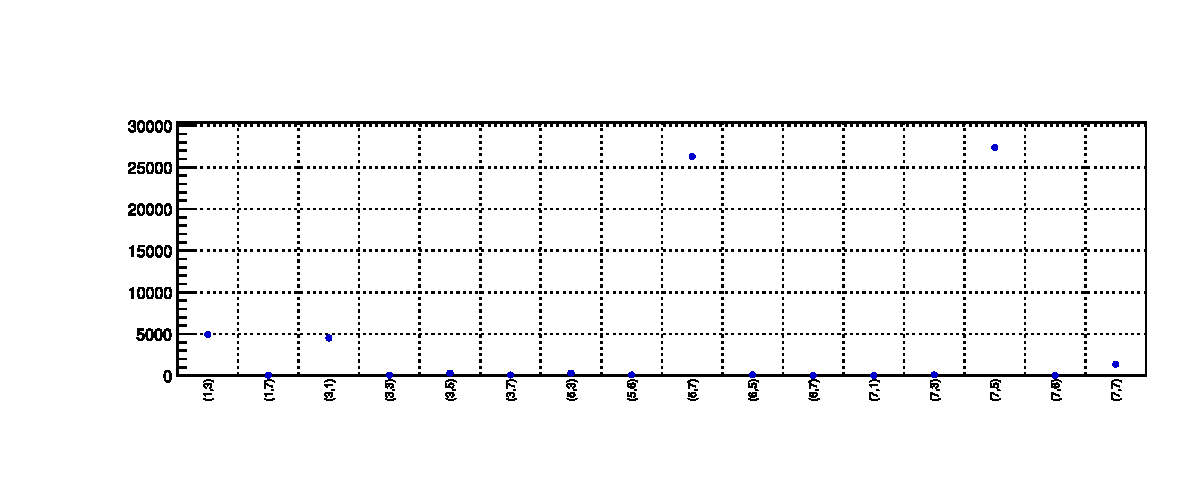
\includegraphics[width=1.08\linewidth]{Pictures/6}
			\end{subfigure}
			
			\vspace{-1.8cm}
			\begin{subfigure}{.49\linewidth}
				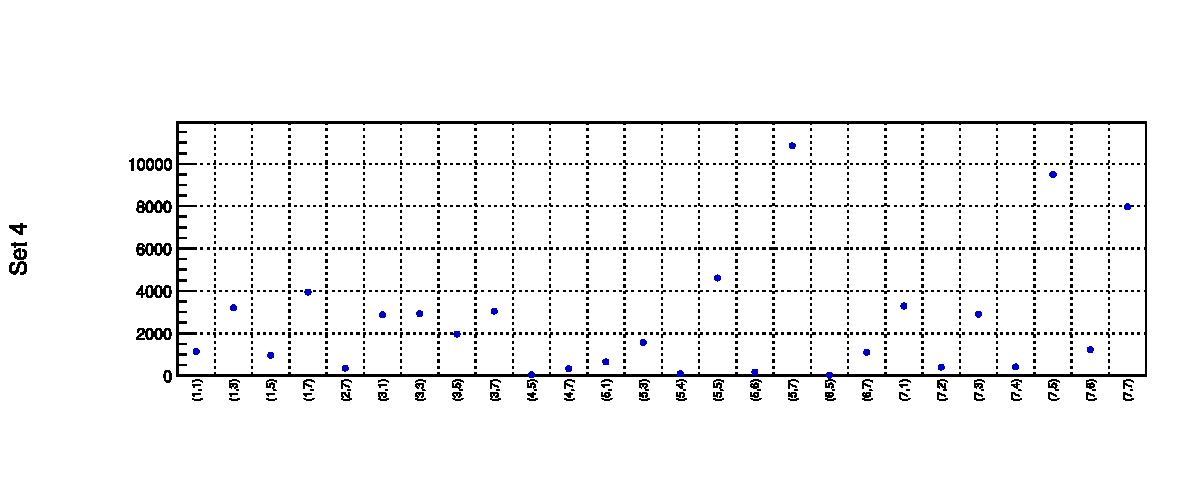
\includegraphics[width=1.08\linewidth]{Pictures/7}
			\end{subfigure}
			\hspace{-.73cm}
			\begin{subfigure}{.49\linewidth}
				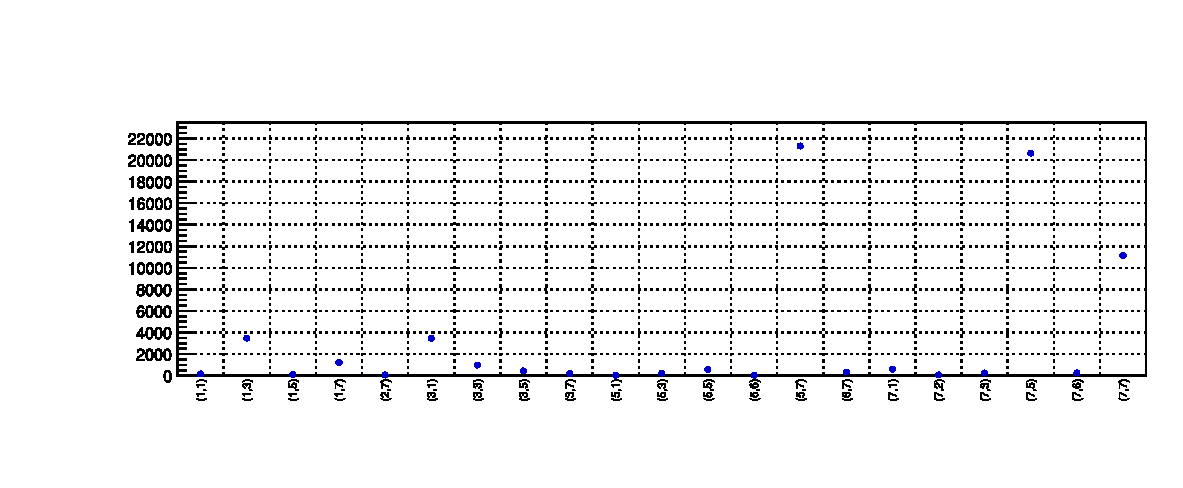
\includegraphics[width=1.08\linewidth]{Pictures/8}
			\end{subfigure}
			\caption{La Figura si legge come una tabella, sulle righe ci sono i diversi set di porte utilizzate, sulle colonne i diversi metodi di risoluzione; sull'asse $x$ di ogni grafico leggiamo gli assegnamenti di $A$ e $B$ osservati; sull'asse $y$ il numero medio di osservazioni per un certo assegnamento, l'errore associato alla misura è la deviazione standard.}
			\label{fig:fact}
		\end{figure}
		
		\par
	\end{landscape}
	\restoregeometry
}